\documentclass{beamer}
%\usepackage[T1]{fontenc}
\usepackage[utf8]{inputenc}
%\usepackage{lmodern}  % Use the Latin Modern font family

\usepackage{latexsym,amsmath,xcolor,bm, amssymb, color, tikz, graphicx, amsthm, mathtools}
\usepackage{algorithm}
\usepackage{algorithmic}
\usepackage{hyperref}
\usepackage{float}     
\usepackage{CJKutf8}
\usepackage{multicol}

\DeclareMathOperator*{\argmax}{arg\,max}
\DeclareMathOperator*{\argmin}{arg\,min}
\DeclareMathOperator{\sign}{sign}
\DeclareMathOperator{\Tr}{Tr}

\makeatletter
\DeclareRobustCommand\onedot{\futurelet\@let@token\@onedot}
\def\@onedot{\ifx\@let@token.\else.\null\fi\xspace}
\def\eg{\emph{e.g}\onedot} 
\def\Eg{\emph{E.g}\onedot}
\def\ie{\emph{i.e}\onedot} 
\def\Ie{\emph{I.e}\onedot}
\def\cf{\emph{c.f}\onedot} 
\def\Cf{\emph{C.f}\onedot}
\def\etc{\emph{etc}\onedot} 
\def\vs{\emph{vs}\onedot}
\def\wrt{w.r.t\onedot} 
\def\dof{d.o.f\onedot}
\def\etal{\emph{et al}\onedot}
\makeatother


\usetheme{Madrid}
\useinnertheme{circles}


\definecolor{ColorUNR}{HTML}{0b2755} 
\usecolortheme[named=ColorUNR]{structure}
%\usecolortheme[named=ColorUNR]{exampleblock}

%\setbeamertemplate{blocks}[rounded][shadow=true]
%\setbeamercolor{block body}{fg=black,bg=white}



%------------------------------------------------------------
%This block of code defines the information to appear in the
%Title page
\title %optional
{Grafos}

\subtitle{Nivel Inicial}

%\subtitle{with applications to persuation and lie production}
% \author % (optional)
% {Author Name}

\author[Mariano Feresin]{Mariano Feresin}

\institute[]{Universidad Tecnológica Nacional - Facultad Regional Santa Fe}
\date[TC 2025]{Training Camp 2025}
\titlegraphic{
\includegraphics[clip,height=2cm,keepaspectratio]{logos/tcarg.jpeg}}

%End of title page configuration block
%------------------------------------------------------------


%------------------------------------------------------------
%The next block of commands puts the table of contents at the 
%beginning of each section and highlights the current section:
\AtBeginSection[]
{
  \begin{frame}
    \frametitle{Outline}
    \tableofcontents[currentsection]
  \end{frame}
}
%------------------------------------------------------------


\begin{document}


%The next statement creates the title page.
\frame{\titlepage}


%------------------------------------------------------------
% Frame de Sponsors, me parece mejor ponerlo al principio
% Antes del índice/contenido

% --- Sponsors Frame 1: Organizador & Diamond Plus ---


% First sponsors frame: Organizador and Diamond Plus
\begin{frame}{Gracias Sponsors!}
    \begin{columns}[t]
        \column{0.5\textwidth}
        \centering
        Organizador\\
        \vspace{0.5cm}
        
\includegraphics[width=1\textwidth,keepaspectratio]{logos/aapc.png}
        
\includegraphics[width=1\textwidth,keepaspectratio]{logos/utn_santafe.png}
        \column{0.5\textwidth}
        \centering
        Diamond Plus\\
        
\includegraphics[width=1\textwidth,keepaspectratio]{logos/GTSlogo.jpeg}
    \end{columns}
\end{frame}

% --- Sponsors Frame 2: Gold & Oro ---

\begin{frame}{Gracias Sponsors!}
    % Platino at the top, full width
    \centering
    Platino\\
    
\includegraphics[width=0.6\textwidth,keepaspectratio]{logos/folder.png}
    
    \vfill
    
    % Gold and Oro at the bottom in two columns
    \begin{columns}[b]
        % Gold column
        \column{0.5\textwidth}
        \centering
        Gold\\
        
\includegraphics[width=0.8\textwidth,keepaspectratio]{logos/neuralsoft.png}
        % Oro column
        \column{0.5\textwidth}
            \centering
        Oro\\
        
\includegraphics[width=0.8\textwidth,keepaspectratio]{logos/jerarquicos.jpg}
    \end{columns}
\end{frame}

% --- Sponsors Frame 3: Aliado ---

\begin{frame}{Gracias Sponsors!}
    \centering
    Aliado\\
    \vspace{1cm}
    
\includegraphics[width=0.6\textwidth,keepaspectratio]{logos/santa_fe_logo_v2.jpg}
\end{frame}


\section{Motivación}

\begin{frame}{Motivación}
	\begin{itemize}
		\item ¿Cómo hace Google Maps para decirte cuál es el camino más rápido?
		\item ¿Como hacemos para eligir qué materias cursar? Algunas tienen correlativas, es decir, hay que hacer una antes que otra.
		\item ¿O cómo Instagram te muestra cuentas de personas que quizás conozcas?
		\item Todas esas cosas tienen algo en común: usan $grafos$.
		\item Un grafo es simplemente una forma de representar cosas (como personas, ciudades, páginas web...) y cómo esas cosas están conectadas entre sí.
	\end{itemize}
\end{frame}

\section{Definiciones}

\begin{frame}{Grafo}
	Grafo $G = (V,E)$
	\begin{itemize}
		\item $V$ es un conjunto de vértices, alias nodos.
		\item Algunos pares de nodos están conectados por aristas, alias ejes. $E$ es el conjunto de aristas.
		\item \textbf{Notación:} $n$ es la cantidad de nodos, $m$ la cantidad de aristas.
	\end{itemize}
	\begin{center}
		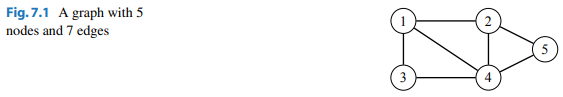
\includegraphics[]{figuras/7.1-grafo.PNG}
	\end{center}
\end{frame}

\begin{frame}{Caminos y Ciclos}
	\begin{itemize}
		\item Un \textbf{camino} lleva de un vértice a otro usando aristas del grafo. Por ejemplo, en la figura, $1 \rightarrow 3 \rightarrow 4 \rightarrow 5$. La longitud de un camino es la cantidad de aristas.
		\item Un \textbf{ciclo} es un camino que empieza y termina en el mismo vértice. Ejemplo: $1 \rightarrow 3 \rightarrow 4$.
	\end{itemize}
	
	\begin{center}
		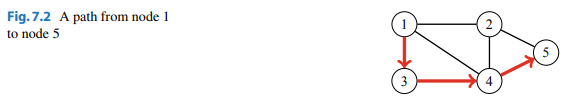
\includegraphics[]{figuras/7.2-camino-simple.PNG}
		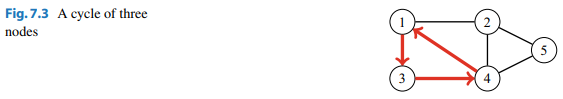
\includegraphics[]{figuras/7.3-ciclo.PNG}
	\end{center}
\end{frame}

\begin{frame}{Conexidad y Componentes}
	\begin{itemize}
		\item Decimos que un grafo es \textbf{conexo} si existe camino entre todo par de vértices.
		\item A cada conjunto maximal de vértice que sea conexo le llamamos \textbf{componente}.
	\end{itemize}
	
	\begin{center}
		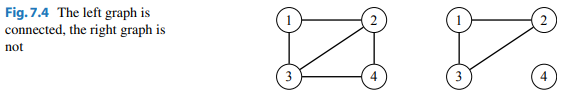
\includegraphics[]{figuras/7.4-conexo.PNG}
		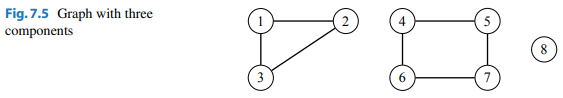
\includegraphics[]{figuras/7.5-componentes.PNG}
	\end{center}
\end{frame}

\begin{frame}{Árboles}
	Un árbol es un grafo:
	\begin{enumerate}
		\item Conexo
		\item Sin ciclos
		\item Con $m = n-1$
	\end{enumerate}
	\begin{center}
		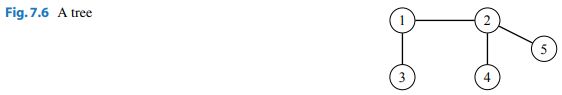
\includegraphics[]{figuras/7.6-arbol.PNG}
	\end{center}
\end{frame}

\begin{frame}{Otros Tipos de Grafos}
	\begin{itemize}
		\item En un grafo \textbf{dirigido} las aristas se pueden recorrer en un único sentido.
		\item En un grafo \textbf{pesado}, cada arista tiene un peso asociado.
	\end{itemize}
	\begin{center}
		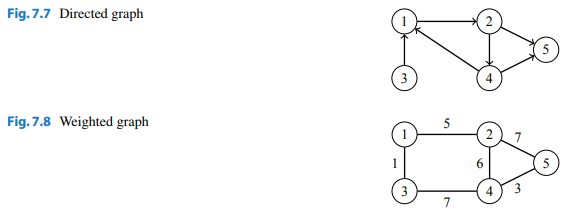
\includegraphics[]{figuras/7.7-dirigido-pesado.PNG}
	\end{center}
\end{frame}

%camino minimo
%grado
%adyacencias, vecinos
%grado entrada/salida
%regular
%completo
%bipartito

\section{Representaciones}

\begin{frame}{Representaciones Comunes}
	Para resolver con grafos, hay que representarlos en la computadora. Elegir la representación que sea más conveniente según características del grafo y qué operaciones necesite realizar el algoritmo. Vemos tres representaciones comunes:
	\begin{enumerate}
		\item Lista de adyacencias.
		\item Lista de aristas.
		\item Matriz de adyacencia.
	\end{enumerate}
\end{frame}

\begin{frame}{Lista de Adyacencias}
	\begin{center}
		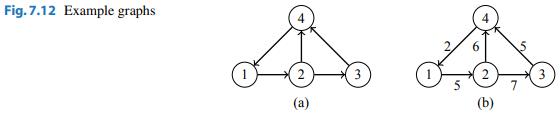
\includegraphics[]{figuras/7.12-grafo-ejemplo.PNG}
		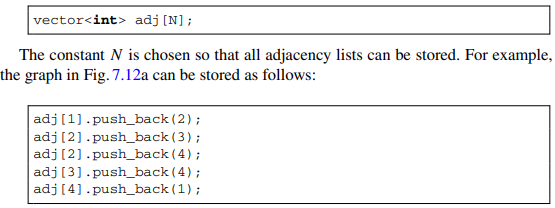
\includegraphics[]{figuras/lista-de-adyacencias.PNG}
	\end{center}
\end{frame}

\begin{frame}{Lista de Adyacencias para Grafo Pesado}
	\begin{center}
		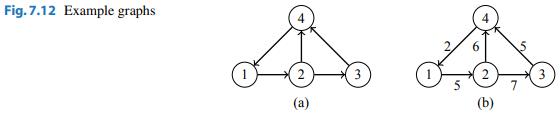
\includegraphics[]{figuras/7.12-grafo-ejemplo.PNG}
		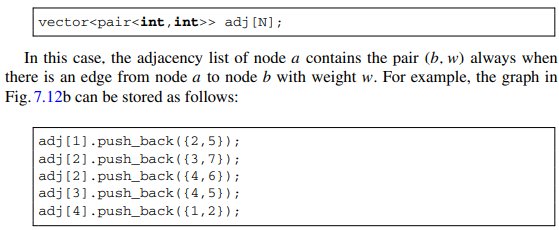
\includegraphics[]{figuras/lista-de-ady-pesado.PNG}
	\end{center}
\end{frame}

\begin{frame}{Lista de Aristas}
	\begin{center}
		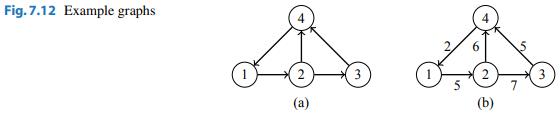
\includegraphics[]{figuras/7.12-grafo-ejemplo.PNG}
		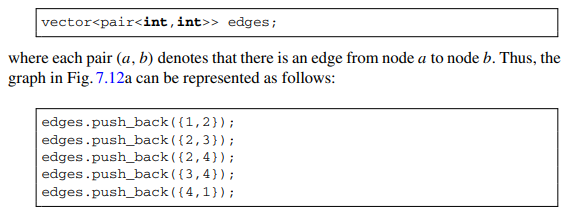
\includegraphics[]{figuras/lista-de-aristas.PNG}
	\end{center}
\end{frame}

\begin{frame}{Lista de Aristas para Grafo Pesado}
	\begin{center}
		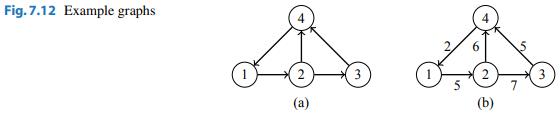
\includegraphics[]{figuras/7.12-grafo-ejemplo.PNG}
		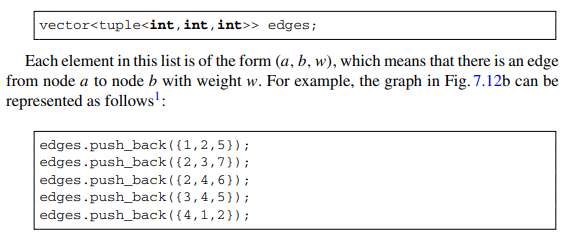
\includegraphics[]{figuras/lista-de-aristas-pesado.PNG}
	\end{center}
\end{frame}

\begin{frame}{Matriz de Adyacencia}
	\begin{center}
		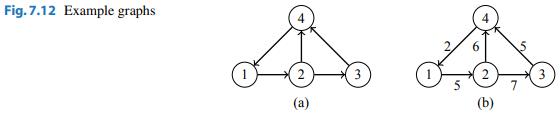
\includegraphics[]{figuras/7.12-grafo-ejemplo.PNG}
		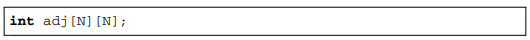
\includegraphics[]{figuras/matriz.PNG}
		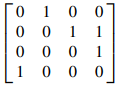
\includegraphics[]{figuras/matriz-no-pesado.PNG}
	\end{center}
	$ady[u][v] = 1$ si y sólo si hay arista de vértice $u$ a $v$.
\end{frame}

\begin{frame}{Matriz de Adyacencia para Grafos Pesados}
	\begin{center}
		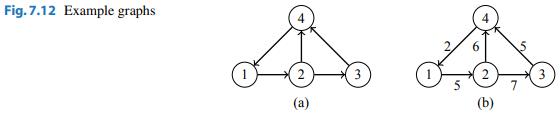
\includegraphics[]{figuras/7.12-grafo-ejemplo.PNG}
		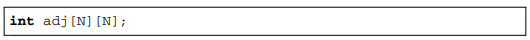
\includegraphics[]{figuras/matriz.PNG}
		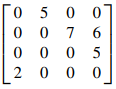
\includegraphics[]{figuras/matriz-pesado.PNG}
	\end{center}
\end{frame}

\section{Recorridos}

\begin{frame}{Recorridos}
	Vemos dos algoritmos fundamentales de grafos: depth-first search (DFS) y breadth-first search (BFS). Ambos recorren todos los nodos que pueden ser alcanzados desde un $v$ inicial, pero en distinto orden.
\end{frame}

\begin{frame}{DFS}
	\begin{itemize}
		\item Recorrido ``en profundidad''.
		\item Sigue por un camino mientras encuentre nodos sin explorar. Luego, vuelve a nodos previos a explorar otras partes del grafo.
	\end{itemize}
	
	\centering
	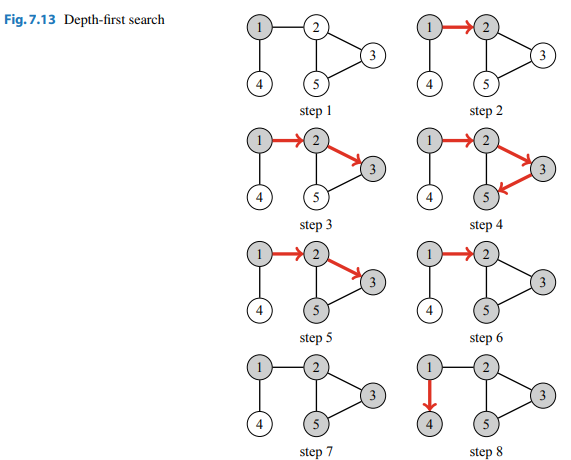
\includegraphics[scale=0.6]{figuras/dfs_ejecucion.PNG}
\end{frame}

\begin{frame}{Código DFS}
	\begin{figure}
		\centering
		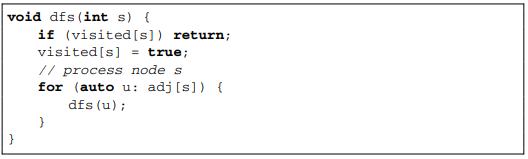
\includegraphics[]{figuras/dfs.PNG}
	\end{figure}
	
	El grafo es representado por $adj$, una lista de adyacencias. Visited es un vector de booleanos.
	
\end{frame}

\begin{frame}{Problema}

	En un curso de programación, los estudiantes quieren organizar un partido de fútbol.
	Para que el partido sea justo, deben dividirse en dos equipos con la misma cantidad de jugadores.
	
	Sin embargo, hay una regla:
	\begin{itemize}
		\item Si dos jugadores comparten una misma habilidad (por ejemplo, son buenos en defensa o patean con la zurda), no pueden estar en el mismo equipo.
	\end{itemize}
	
	La pregunta es:
	¿Es posible formar los equipos de manera que todos puedan jugar respetando esa regla?
\end{frame}

\begin{frame}{Colorear un grafo}
	\begin{itemize}
		\item Colorear un grafo es asignar a cada nodo un $color$ de manera que no existan dos nodos adyacentes del mismo color.
		\item Un grafo es \textbf{bipartito} si es posible colorear el grafo usando dos colores.
		\item Un grafo es bipartito cuando no contiene un ciclo con una cantidad impar de aristas
	\end{itemize}
	
	\centering
	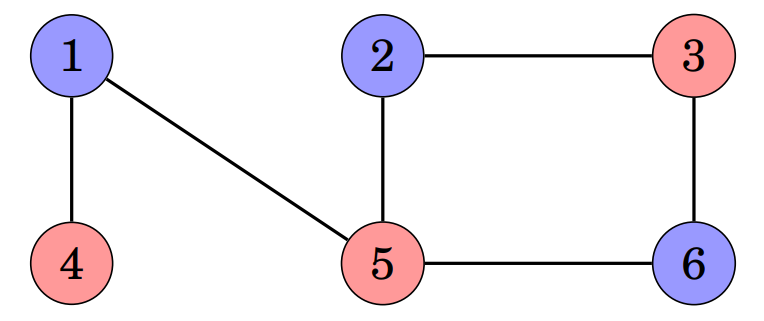
\includegraphics[scale=0.3]{figuras/grafo-bipartito.PNG}
\end{frame}

\begin{frame}{Código Bipartito}
	\begin{flushleft}
	Para saber si un grafo es bipartito utilizamos DFS, asignamos un primer nodo con un color arbitrario, a los vecinos de este el color contrario y llamamos recursivamente. Si nos encontramos 
	con un vecino del mismo color el grafo no es bipartito.
	\end{flushleft}
	\centering
	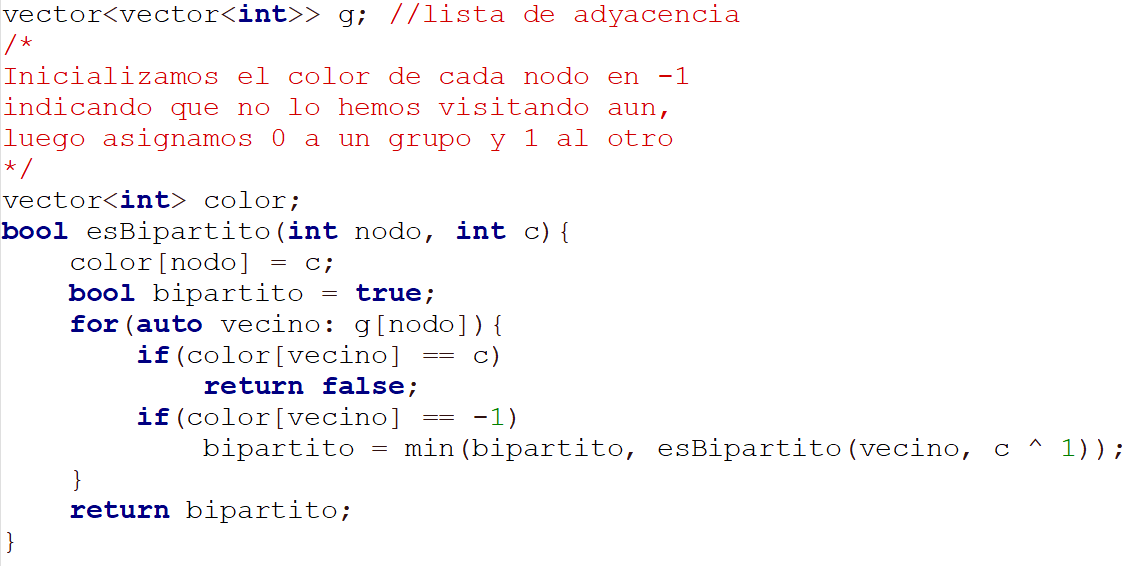
\includegraphics[scale=0.4]{figuras/codigo-bipartito.PNG}
\end{frame}

\begin{frame}{BFS}
	\begin{itemize}
		\item Recorrido ``a lo ancho''.
		\item Va explorando el grafo en orden creciente de distancia desde un origen.
	\end{itemize}
	
	\centering
	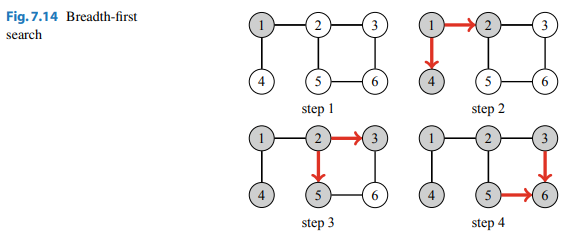
\includegraphics[scale=0.7]{figuras/bfs_ejecucion.PNG}
\end{frame}

\begin{frame}{Código BFS}
	\centering
	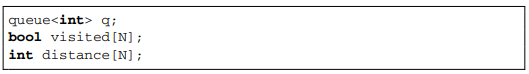
\includegraphics[]{figuras/estructuras bfs.PNG}
	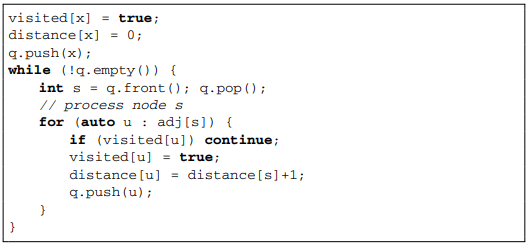
\includegraphics[]{figuras/bfs.PNG}
\end{frame}

\section{Camino Mínimo}

\begin{frame}{Miremos un poco}
	\begin{itemize}
		\item Volvamos al ejemplo del recorrido BFS
	\end{itemize}
	
	\centering
	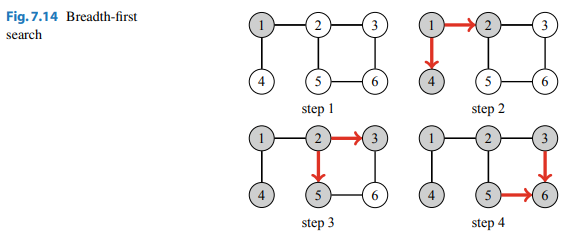
\includegraphics[scale=0.7]{figuras/bfs_ejecucion.PNG}
	\begin{itemize}
		\item ¿Qué tienen en común los nodos 2 y 4?
		\item ¿Y los nodos 3 y 5?
	\end{itemize}
\end{frame}

\begin{frame}{Camino Mínimo}
	\begin{itemize}
		\item Un problema recurrente es encontrar el camino de mínimo costo entre dos vértices.
		\item Hoy menciono cuatro algoritmos para resolver este problema:
		\begin{itemize}
			\item BFS,
			\item Bellman Ford,
			\item Dijkstra y
			\item Floyd-Warshall.
		\end{itemize}
	\end{itemize}
\end{frame}

\begin{frame}{Bellman Ford}
	\begin{itemize}
		\item En grafos pesados necesitamos otros algoritmos.
		\item Bellman Ford calcula camino mínimo desde un vértice hacia todos.
		\item Si hay ciclos negativos, el problema del camino mínimo se indefine. Bellman Ford detecta si hay un ciclo negativo.
		\item \textbf{Invariante:} luego de su k-ésima iteración, calcula la distancia mínima a todo $v$ usando a lo sumo $k$ aristas\footnote{En realidad, no exactamente...}.
		\item \textbf{Complejidad:} $O(nm)$.
	\end{itemize}
\end{frame}

\begin{frame}{Código Bellman Ford}
	\centering
	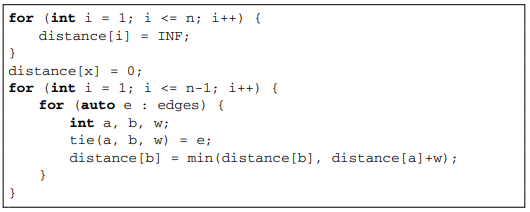
\includegraphics[]{figuras/bellman_ford.PNG}
\end{frame}

\begin{frame}{Detectando ciclos negativos}
	\begin{itemize}
		\item ¿Cómo detectamos un ciclo negativo?
		
		\item \textbf{Intuición:} Sabemos que si no hay ciclos negativos, un camino minimo tiene a los sumo $n-1$ aristas, es decir, como mucho pasa 1 vez por cada nodo del grafo, si tendria más aristas significaría que pasamos dos veces por un nodo lo cual no seria óptimo.
		
		\item Una vez que terminamos las $n-1$ iteraciones de Bellman-Ford, hacemos una pasada extra.
		
		\item Si en esa última pasada alguna arista puede seguir relajándose, significa que hay un ciclo con peso negativo
		
		\item Podríamos seguir mejorando distancias infinitamente. Esa es la señal de que existe un ciclo negativo.	
	\end{itemize}
	\centering
	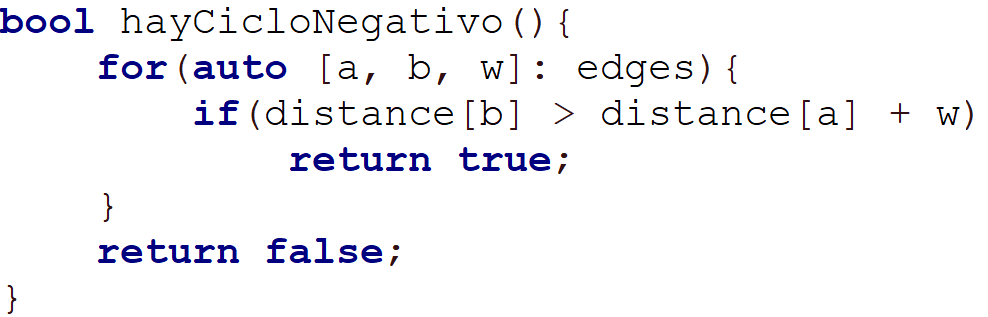
\includegraphics[scale=0.3]{figuras/ciclo-negativo-codigo.PNG}
\end{frame}

\begin{frame}{Dijkstra}
	\begin{itemize}
		\item Camino mínimo de uno a todos.
		\item Requiere que el costo de las aristas sea no negativo.
		\item \textbf{Invariante:} antes de la k-ésima iteración, calcula correctamente la distancia hacia los $k$ vértices más cercanos al origen.
		\item En cada iteración, toma al vértice no procesado que esté a distancia mínima del origen.
		\item \textbf{Complejidad:} $O(min\{n^2, m\, lg\, n\})$.
	\end{itemize}
\end{frame}

\begin{frame}{Código Dijkstra}
	\centering
	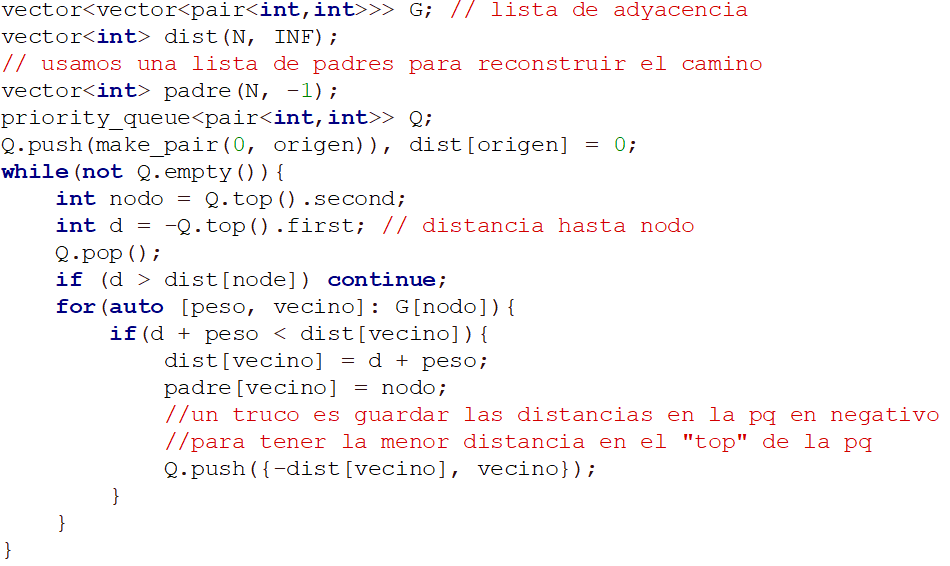
\includegraphics[scale=0.47]{figuras/codigo-dijkstra.PNG}
\end{frame}

\begin{frame}{Floyd-Warshall}
	\begin{itemize}
		\item Computa distancia entre todo par de vértices.
		\item \textbf{Invariante:} luego de la k-ésima iteración, computa los caminos k-internos\footnote{Decimos que un camino es k-interno si todos los vértices intermedios (o sea, exluyendo al primero y al último) tienen un índice menor o igual a k} mínimos.
		\item \textbf{Complejidad:} $O(n^3)$.
	\end{itemize}
\end{frame}

\begin{frame}{Código Floyd-Warshall}
	\centering
	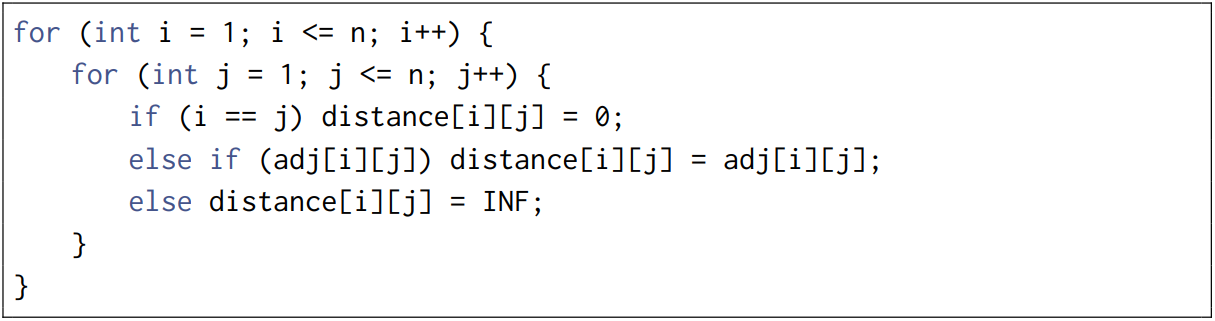
\includegraphics[scale=0.35]{figuras/codigo-floyd-1.PNG}
	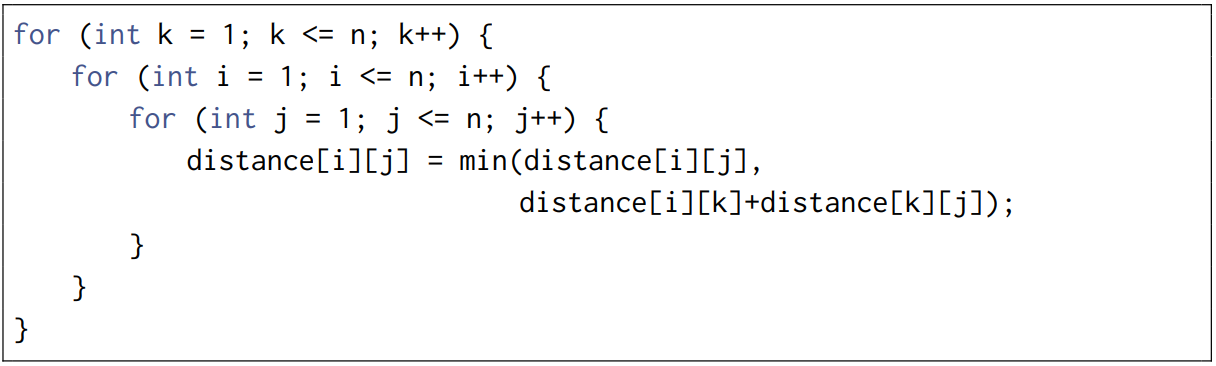
\includegraphics[scale=0.35]{figuras/codigo-floyd-2.PNG}
\end{frame}

\begin{frame}{Tips}
	\begin{itemize}
		\item Los algoritmos de 1 a todos se pueden transformar en algoritmos para encontrar caminos de todos a uno (revirtiendo el sentido de los ejes).
		\item Se pueden usar para computar caminos de todos a todos (haciendo $n$ ejecuciones del algoritmo, una desde cada origen).
		\item Pueden usar los algoritmos para calcular distancias y también para obtener el árbol de caminos mínimos. Ojo, puede haber varios caminos mínimos, sólo alguno pertenece a este árbol.
		\item Si sienten que les falta información en el grafo, consideren agregar vértices para codificar esa información faltante.
		\item Se pueden correr estos algoritmos teniendo mas de un nodo origen
	\end{itemize}
\end{frame}

%truquitos de modelado?

%\section{Grafo Dirigido Acíclico?}

%\section{Grafo de Función?}

\section{Árbol Generador Mínimo}

\begin{frame}{Árbol Generador Mínimo}
	\begin{itemize}
		\item Otro problema recurrente.
		\item Un árbol generador (AG) contiene a todos los nodos del grafo, a algunas ($n-1$) de sus aristas y conecta a todos los vértices.
		\item El costo de un AG es la suma de los costos de las aristas que contiene.
		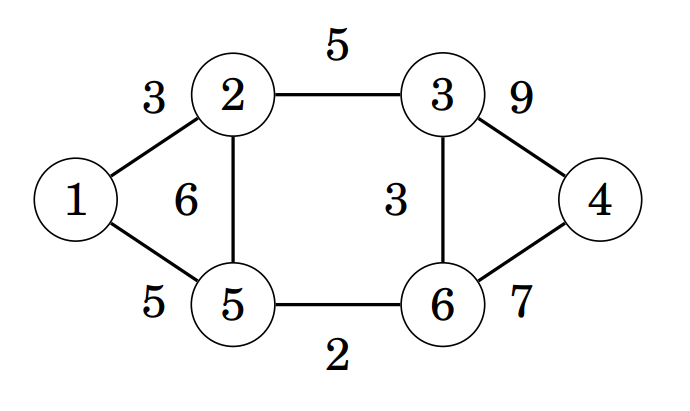
\includegraphics[scale=0.30]{figuras/grafo-kruskal-1.PNG}
		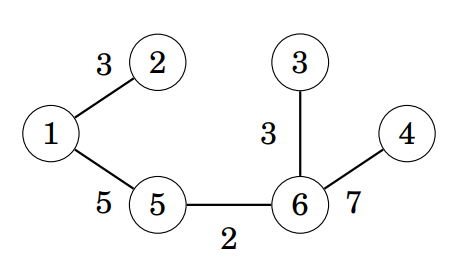
\includegraphics[scale=0.42]{figuras/grafo-kruskal-2.PNG}
	\end{itemize}
\end{frame}

\begin{frame}{Union Find}
	\begin{itemize}
		\item Si bien esta no es una clase de estructura de datos, la estructura Union Find va a ser útil para encontrar el árbol generador mínimo de un grafo.
		\item Union Find es una estructura que mantiene una colección de conjuntos. Los conjuntos son disjuntos, es decir, ningun elemento pertenece a más de un conjunto.
		\item Cada conjunto tine un elemento que es el representante de este y hay una cadena desde cada elemento del conjunto hasta el representante.
	\end{itemize}
	\centering
	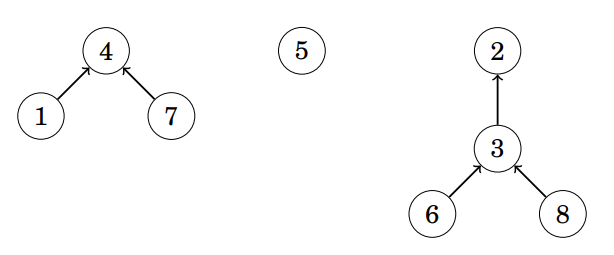
\includegraphics[scale=0.50]{figuras/union-find.PNG}
\end{frame}

\begin{frame}{Union Find}
	\begin{itemize}
		\item Si bien esta no es una clase de estructura de datos, la estructura Union Find va a ser útil para encontrar el árbol generador mínimo de un grafo.
		\item Union Find es una estructura que mantiene una colección de conjuntos. Los conjuntos son disjuntos, es decir, ningun elemento pertenece a más de un conjunto.
		\item Cada conjunto tine un elemento que es el representante de este y hay una cadena desde cada elemento del conjunto hasta el representante.
	\end{itemize}
	\centering
	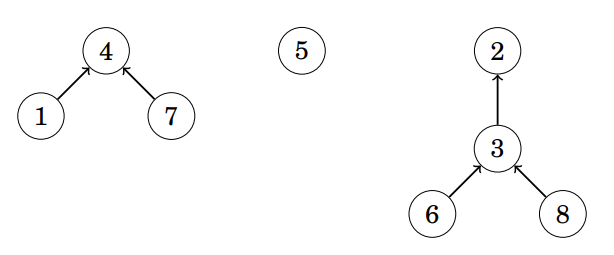
\includegraphics[scale=0.50]{figuras/union-find.PNG}
\end{frame}

\begin{frame}{Union Find}
	Union Find soporta dos tipos de operaciones: 
	\begin{itemize}
		\item $unite:$ nos permite unir dos conjuntos
		\item $find:$ nos permite encontrar el representante de un elemento
		\item No vamos a analizar la complejidad de estas operaciones pero pueden asumir que son prácticamente constantes.\footnote{Para los curiosos pueden más leer sobre esto acá: codeforces.com/blog/entry/98275}
	\end{itemize}

\end{frame}

\begin{frame}{Código Union Find}
	\begin{itemize}
		\item Encontrar el representante de un elmento es simplemente recorrer su cadena de representantes
		\item Para unir dos conjuntos conectamos el reprensentante del conjunto mas chico al representante del conjunto mas grande para así lograr que la estructura sea eficiente.
	\end{itemize}
	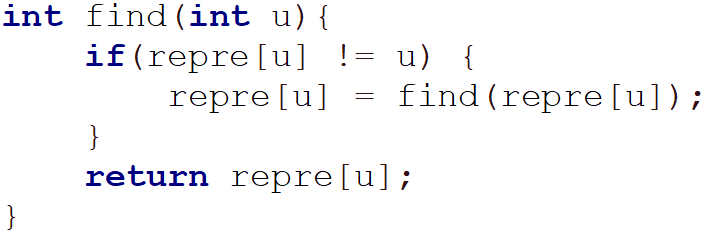
\includegraphics[scale=0.30]{figuras/codigo-find.PNG}
	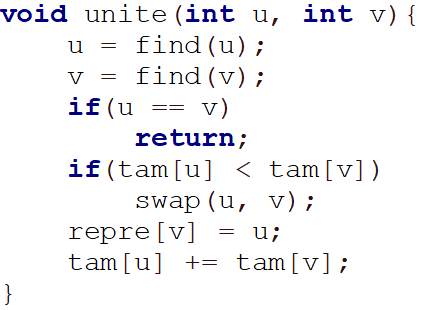
\includegraphics[scale=0.40]{figuras/codigo-unite.PNG}
\end{frame}

\begin{frame}{Implementación Kruskal}
	Ahora que conocemos la estructura Union Find podemos ver como encontrar el árbol generador mínimo de un grafo.
	\begin{itemize}
		\item Se ordenan las arista por costo, de menor a mayor.
		\item Se procesa cada arista $u,v$: si $u$ y $v$ están en distintas componentes, se agrega la arista al bosque.
		\item Para responder eficientemente si están en la misma componente, usamos la estructura union-find.
	\end{itemize}
	\centering
	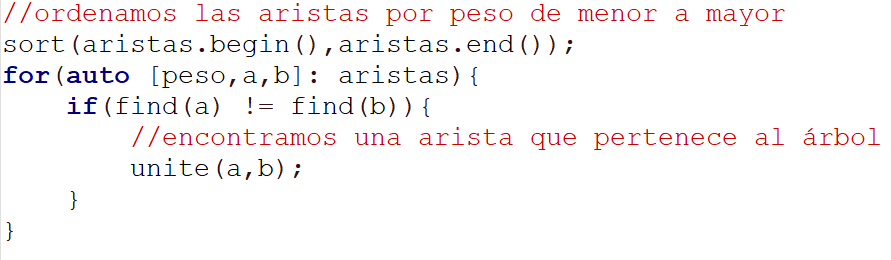
\includegraphics[scale=0.40]{figuras/codigo-kruskal.PNG}
\end{frame}


\section{Cierre}

\begin{frame}{Referencias}
	Les dejo el libro Guide to Competitive Programming, de Antti Laaksonen.
	\begin{itemize}
		\item https://cses.fi/book/book.pdf
	\end{itemize}
	En la sección de grafos van a poder ver mas sobre los temas que vimos hoy y chusmear mas cosas sobre grafos.
\end{frame}


\begin{frame}{Problemas para practicar}
	\begin{itemize}
		\item Les dejo problemas de CSES:
		\begin{itemize}
			\item \url{https://cses.fi/problemset/task/1667}
			\item \url{https://cses.fi/problemset/task/1671}
			\item \url{https://cses.fi/problemset/task/1669}
			\item \url{https://cses.fi/problemset/task/1672}
			\item \url{https://cses.fi/problemset/task/1673}
			\item \url{https://cses.fi/problemset/task/1195}
			\item \url{https://cses.fi/problemset/task/1675}
			\item \url{https://cses.fi/problemset/task/1676}
		\end{itemize}
	\end{itemize}
\end{frame}

\begin{frame}{Consultas}
	Pueden consultarme durante estas semanas, o me pueden escribir al Telegram:
	\begin{itemize}
		\item @marianoferesin
	\end{itemize}
	%\bibliography{ref}
\end{frame}

\begin{frame}{Saludo}
	\centering
	Gracias a todos por su atención y mucha suerte en el contest de la tarde.
	%\bibliography{ref}
\end{frame}

\end{document}
